\FloatBarrier
\begin{figure}[!h]
\centering
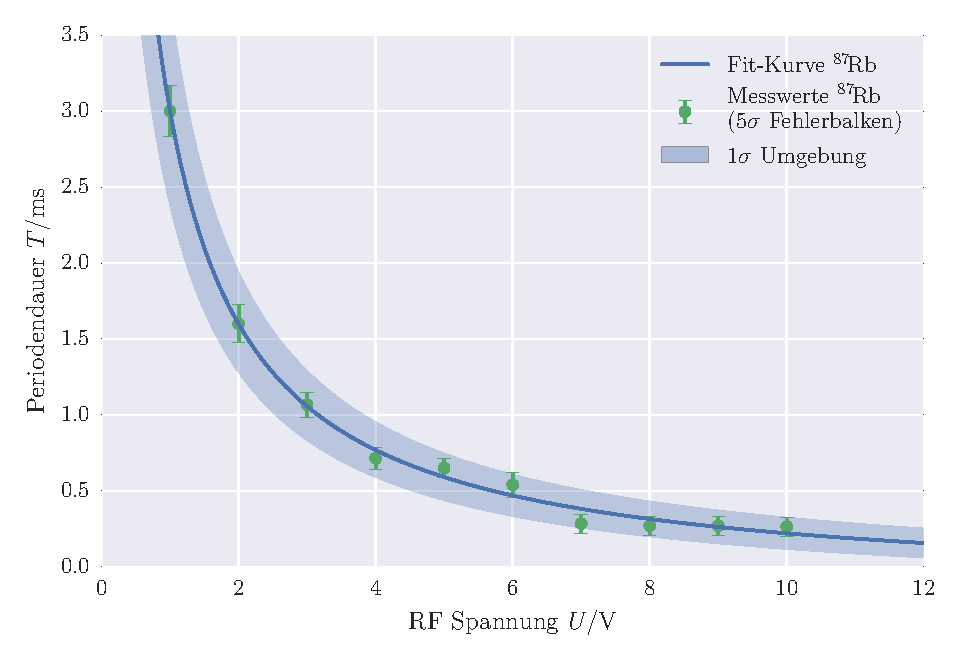
\includegraphics[scale=.85]{../Grafiken/Transienteneffekt_Rubidium_87.pdf}
\caption{In Abhängigkeit der RF-Spannung dargestellte Periodendauern der Relaxation
	für das Isotop ${}^{87}\!$Rb. Die Fehlerbalken der Messwerte wurden verfünffacht, 
	um sichtbar zu sein. Zusätzlich ist die hyperbolische Ausgleichskurve für die Messwerte
	dargestellt. \label{fig:transienteneffekt_rubidium_87}}
\end{figure}
\FloatBarrier